
%===================================================================================================
%	DOCUMENT DEFINITION
%===================================================================================================

%we use article class because we want to fully customize the page and dont use a cv template
\documentclass[10pt,a4paper]{article}	

%---------------------------------------------------------------------------------------------------
%	ENCODING
%---------------------------------------------------------------------------------------------------

%we use utf8 since we want to build from any machine
\usepackage[utf8]{inputenc}		

%---------------------------------------------------------------------------------------------------
%	LOGIC
%---------------------------------------------------------------------------------------------------

% provides \isempty test
\usepackage{xifthen}

%---------------------------------------------------------------------------------------------------
%	FONT
%---------------------------------------------------------------------------------------------------

% some tex-live fonts - choose your own

%\usepackage[defaultsans]{droidsans}
%\usepackage[default]{comfortaa}
%\usepackage{cmbright}
\usepackage[default]{raleway}
%\usepackage{fetamont}
%\usepackage[default]{gillius}
%\usepackage[light,math]{iwona}
%\usepackage[thin]{roboto}
\usepackage{hyperref}

% set font default
\renewcommand*\familydefault{\sfdefault} 	
\usepackage[T1]{fontenc}

% more font size definitions
\usepackage{moresize}		

%---------------------------------------------------------------------------------------------------
%	PAGE LAYOUT  DEFINITIONS
%---------------------------------------------------------------------------------------------------

%debug page outer frames
%\usepackage{showframe}			

%define page styles using geometry
\usepackage[a4paper]{geometry}		

% for example, change the margins to 2 inches all round
\geometry{top=1.75cm, bottom=-.6cm, left=1.5cm, right=1.5cm} 	

%use customized header
\usepackage{fancyhdr}		
\pagestyle{fancy}

%less space between header and content
\setlength{\headheight}{-5pt}		

%customize entries left, center and right
\lhead{}
\chead{\small{
  Dipayan Roy $\cdot$ 
  Computer Science Undergraduate $\cdot$ 
  Kolkata,India $\cdot$ 
  \textcolor{sectcol}{\textbf{\href
  {mailto:dr13@iitbbs.ac.in}
  {dr13@iitbbs.ac.in}}} $\cdot$
  +91-7077-1037-91
}}
\rhead{}

%indentation is zero
\setlength{\parindent}{0mm}

%---------------------------------------------------------------------------------------------------
%	TABLE /ARRAY DEFINITIONS
%--------------------------------------------------------------------------------------------------- 

%for layouting tables
\usepackage{multicol}			
\usepackage{multirow}

%extended aligning of tabular cells
\usepackage{array}
\newcolumntype{x}[1]{>{\raggedleft\hspace{0pt}}p{#1}}

%---------------------------------------------------------------------------------------------------
%	GRAPHICS DEFINITIONS
%--------------------------------------------------------------------------------------------------- 

%for header image
\usepackage{graphicx}

%for floating figures
\usepackage{wrapfig}
\usepackage{float}
%\floatstyle{boxed} 
%\restylefloat{figure}

%for drawing graphics		
\usepackage{tikz}				
\usetikzlibrary{shapes, backgrounds,mindmap, trees}

%---------------------------------------------------------------------------------------------------
%	Color DEFINITIONS
%--------------------------------------------------------------------------------------------------- 

\usepackage{color}

%accent color
\definecolor{sectcol}{RGB}{90,90,120}

%dark background color
\definecolor{bgcol}{RGB}{110,110,110}

%light background / accent color
\definecolor{softcol}{RGB}{225,225,225}

%===================================================================================================
%	DEFINITIONS
%===================================================================================================

%---------------------------------------------------------------------------------------------------
% 	HEADER
%---------------------------------------------------------------------------------------------------

% remove top header line
\renewcommand{\headrulewidth}{0pt} 

%remove botttom header line
\renewcommand{\footrulewidth}{0pt}	  	

%remove pagenum
\renewcommand{\thepage}{}	

%remove section num		
\renewcommand{\thesection}{}			

%---------------------------------------------------------------------------------------------------
% 	ARROW GRAPHICS in Tikz
%---------------------------------------------------------------------------------------------------

% a six pointed arrow poiting to the left
\newcommand{\tzlarrow}{(0,0) -- (0.2,0) -- (0.3,0.2) -- (0.2,0.4) -- (0,0.4) -- (0.1,0.2) -- cycle;}	

% include the left arrow into a tikz picture
% param1: fill color
%
\newcommand{\larrow}[1]{
  \begin{tikzpicture}[scale=0.58]
    \filldraw[fill=#1!100,draw=#1!100!black]  \tzlarrow
  \end{tikzpicture}
}

% a six pointed arrow poiting to the right
\newcommand{\tzrarrow}{ (0,0.2) -- (0.1,0) -- (0.3,0) -- (0.2,0.2) -- (0.3,0.4) -- (0.1,0.4) -- cycle;}

% include the right arrow into a tikz picture
% param1: fill color
%
\newcommand{\rarrow}{
  
\begin{tikzpicture}[scale=0.7]
    \filldraw[fill=sectcol!100,draw=sectcol!100!black] \tzrarrow
  \end{tikzpicture}
}
%---------------------------------------------------------------------------------------------------
%	custom sections
%---------------------------------------------------------------------------------------------------

% create a coloured box with arrow and title as cv section headline
% param 1: section title
%
\newcommand{\cvsection}[1]{
  \vspace{10pt}
  \colorbox{sectcol}{\mystrut \makebox[1\linewidth][l]{
    \larrow{bgcol} \hspace{-8pt} \larrow{bgcol} \hspace{-8pt} 
    \larrow{bgcol}\textcolor{white}{\textbf{#1}}\hspace{4pt}
    \vspace{5pt}
  }}\\
}

%create a coloured arrow with title as cv meta section section
% param 1: meta section title
%
\newcommand{\metasection}[2]{
  \begin{tabular*}{1\textwidth}{p{2.4cm} p{11cm}}
    \larrow{bgcol} \normalsize{\textcolor{sectcol}{#1}}&#2\\[10pt]
  \end{tabular*}
}

%---------------------------------------------------------------------------------------------------
%	 CV EVENT
%---------------------------------------------------------------------------------------------------

% creates a stretched box as cv entry headline followed by two paragraphs
% param 1:	event time i.e. 2014 or 2011-2014 etc.
% param 2:	event name (what did you do?)
% param 3:	institution (where did you work / study)
%
\newcommand{\cvevent}[3]{
  \begin{tabular*}{1\textwidth}{p{2.5cm} p{10.5cm} x {4.0cm}}
    \textcolor{bgcol}{#1} & \textbf{#2} & \vspace{2.5pt}\textcolor{sectcol}{#3}
  \end{tabular*}
  \vspace{-10pt}
  \textcolor{softcol}{\hrule}
  \vspace{10pt}
}

% creates a stretched box as cv entry detail 
% param 1:	information describing the event
%
\newcommand{\cvdetail}[1]{
  \begin{tabular*}{1\textwidth}{p{2.5cm} p{14.5cm}}
    & \larrow{bgcol}  #1\\ [3pt]
  \end{tabular*}
}
\newcommand{\cvpoint}[1]{

  \begin{tabular*} {1\textwidth}{p{1.0cm} p{14.5cm}}
    & \larrow{bgcol}  #1\\ [3pt] &\vspace{0.5pt}
  \end{tabular*}
}

%---------------------------------------------------------------------------------------------------
% CUSTOM STRUT FOR EMPTY BOXES
%---------------------------------------------------------------------------------------------------
\newcommand{\mystrut}{\rule[-.3\baselineskip]{0pt}{\baselineskip}}

%===================================================================================================
%	DOCUMENT CONTENT
%===================================================================================================
\title{resume}
\begin{document}

% use our custom fancy header definitions
\pagestyle{fancy}	

%---------------------------------------------------------------------------------------------------
%	TITLE HEADLINE
%---------------------------------------------------------------------------------------------------

\vspace{-20pt}

% use this for single words, e.g. CV or RESUME etc.
\hspace{-0.25\linewidth}\colorbox{bgcol}{
  \makebox[1.5\linewidth][c]{
    \HUGE{\textcolor{white}{\textsc{Dipayan Roy}}} 
    \textcolor{sectcol}{\rule[-1mm]{1mm}{0.9cm}} 
    \HUGE{\textcolor{white}{\textsc{Resume}}}
  }
}

%---------------------------------------------------------------------------------------------------
%	HEADER IMAGE
%---------------------------------------------------------------------------------------------------

\begin{figure}[H]
\begin{flushright}
	\vspace{5pt}
  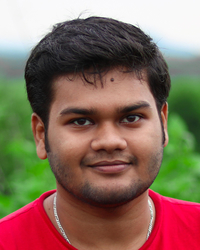
\includegraphics[width=0.2\linewidth]{dipayan.jpg}
\end{flushright}
\end{figure}

%---------------------------------------------------------------------------------------------------
%	META SECTION
%---------------------------------------------------------------------------------------------------

\vspace{-140pt}

\metasection{Status:}{Student at IIT Bhubaneshwar, Undergraduate of Computer Science from School of Electrical Sciences}
\metasection{Skills:}{C, Python, Java, C++, Database(SQL,My-SQL,Oracle), PHP, HTML, Javascript, CSS} 
\metasection{Interests:}{Cryptography, Operating Systems, Database Management, Data       Analytics, Algorithms, Networking, Machine Learning}
\metasection{Activities:}{Football, Table Tennis, Cricket, Basketball, Reading, Music, Coding}

%---------------------------------------------------------------------------------------------------
%	ABOUT ME
%---------------------------------------------------------------------------------------------------

\cvsection{About Me}

Passionate coder who likes to invest his time on knowing about cutting edge technologies. Also dedicated and motivated engineering undergraduate seeking internship opportunity, eager to get exposures to real-world client challenges and solutions, also work side-by-side a dedicated team to get exposures to international projects and solve some existing problems.

%===================================================================================================
%	CV SECTIONS AND EVENTS (MAIN CONTENT)
%===================================================================================================

%---------------------------------------------------------------------------------------------------
%	PROJECTS
%---------------------------------------------------------------------------------------------------
\cvsection{Projects}

\cvevent{'17/02 - now}{BT Project}{IIT Bhubaneswar}
\cvdetail{Topic: Pen-Tablet-Interface based handwriting recognition system}
\cvdetail{Use a pattern recognisation - machine learning techinique to come up with an workable module to recognise a given handwriting manuscript}
\cvdetail{Some features includes use of stylus for online recognisation of characters or use of camera as scanner to get input of handwriting for off-line input,transcribing a
language message represented in a spatial form of graphical
marks into a computer text,using pattern recognisation to build a robust and reliable recognisation system.}
\cvdetail{The project is in its building stages and needs lots of careful implementation of researches as it is one of growing field of interests recently}
\cvdetail{This project is being supervised by Prof. Dr. NB Puhan}

\cvevent{'16/08 - '16/12}{Database Management Project}{IIT Bhubaneswar}

\cvdetail{The aim of this project was to built an on-line ticketing system of Indian railways}
\cvdetail{Some features included data abstraction and independence, implementation of Data security, a locking mechanism for concurrent access, use of Processes and Triggers for efficient data handler, robust data integrity capability, introduction of uniform administration procedures for data, simple access using a standard API}
\cvdetail{Languages used were HTML, PHP, CSS, Javascript, Database(My-SQL), Server(XAMPP)}
\cvdetail{This project was done under the guidance of Asst. Prof. Dr PL Bera and Batakrishna Tripathy(TA) in group of 2. }


\cvevent{'15/08 - '15/12}{Seminar Project}{IIT Bhubaneswar}
\cvdetail{Seminar presentation on the detailed study of “Happy Birthday Paradox” and the modus operandi of Birthday Attacks}
\cvdetail{The main aim was to extensively study a cryptographic attack that exploits the mathematics in probability theory and showing a relative study on its probability of being exploited.}
\cvdetail{This project was supervised by Prof. DP Dogra}

%---------------------------------------------------------------------------------------------------
%	EDUCATION SECTION
%---------------------------------------------------------------------------------------------------

\pagebreak
\thispagestyle{plain}


\cvsection{Education}

\cvevent{2014 - 2018}{Bachelor of Technology,Major-Computer Science}{IIT Bhubaneswar}
\cvdetail{Expected CGPA: 6.53/10 (including laterals) }
\cvdetail{Major Courses: Operating Systems, Computer Networks, Database Management Systems, Programming Languages, Design and Analysis of Algorithms, Formal Automata Theory, Digital Hardware Design and Computer Architecture, Discrete Mathematical Structures.}
\cvdetail{Lateral Courses: Digital Signal Processing, Signal and Systems, Electrical Technology, International Business, Managerial Economics, English for Communication/Learning English. }
\cvdetail{Participated in various technical competitions like Remote Control Car, Robo Kick-Off, etc}

\cvevent{2012 - 2014}{Higher Secondary,Science}{Shiv Jyoti Sr. Sec. Convent School}
\cvdetail{Board: CBSE}
\cvdetail{Percentage: 87.8\% }
\cvdetail{Awarded merit scholarship in intermediate studies for above 90\% marks in matriculation.}


\cvevent{2012}{Secondary}{Modern English Academy}
\cvdetail{Board: ICSE}
\cvdetail{Percentage: 91.6\% }
\cvdetail{Represented school in different inter-school debates, General Knowledge competitions, National and International Olympiads.}

%---------------------------------------------------------------------------------------------------
%	POSITION OF RESPONSIBILITY 
%---------------------------------------------------------------------------------------------------

\cvsection{Position of Responsibility}
\cvpoint{Presently Working as \textbf{Event Management and Hospitality Core Head} at Wissenaire 2017, The Annual Techno ‐ Management fest of IIT Bhubaneswar.}
\cvpoint{Former \textbf{Wing Councillor of Hostels} at IIT Bhubaneswar.}
\cvpoint{Former \textbf{core team member} of Events Management Team, Wissenaire-2016}
\cvpoint{Member of the \textbf{organising team} of Hostel Day, Institute Day, Fresher's and Farewell's Party}

%---------------------------------------------------------------------------------------------------
%	EXTRA CURRICULAR ACTIVITIES
%---------------------------------------------------------------------------------------------------

\cvsection{Extracurricular Activity}

\cvpoint{Actively taken part in fitness and sports, mainly in playing \textbf{Soccer}, represented the college in many inter-college tournaments and matches.}
\cvpoint{Have actively taken interest to contribute towards the society through \textbf{Souls-for-Solace}, the social welfare society, which takes up initiative to help the society by donating the need.}
\cvpoint{Have actively taken part in Fine Arts Society, \textbf{Kalakriti}, contributed many drawings, doodles and designs for decorations on various special ocassions.}
\cvpoint{Contributing to the society by teaching the underpriviledged kids in primary/middle schools under '\textbf{Unnyat-Bharat-Abhiyan}' and cleaning up the streets under  '\textbf{Swatch-Bharat-Abhiyan}'.}



%---------------------------------------------------------------------------------------------------
%	ARTIFICIAL FOOTER (fancy footer cannot exceed linewidth) 
%---------------------------------------------------------------------------------------------------

\null
\vspace*{\fill}
\hspace{-0.25\linewidth}\colorbox{bgcol}{
  \makebox[1.5\linewidth][c]{
    \mystrut \small 
    \textcolor{white}{
      \href{https:/www.linkedin.com/in/roy-dipayan/}
      {Linked In: roy-dipayan}
    } $\cdot$ 
    \textcolor{white}{
      \href{https://github.com/roydipayan003}
      {GitHub: roydipayan003}
    }$\cdot$ 
    \textcolor{white}{
      \href{https://www.facebook.com/iamdipayan}
     	 {Facebook: iamdipayan}
     }
  }
}

%===================================================================================================
%	DOCUMENT END
%===================================================================================================
\end{document}
